% tutorial_basis.tex — DRIVER for the RecoCrysp tutorial "basis" document.
%
% This file only sets up the document and \input{}s the section sources from
% tbsrc/. Each section is developed independently in its own tbsrc/*.tex file
% so they can be written and reviewed one at a time. See ../PLAN.md for the
% full plan, the section outline, and the technical decisions behind the text.
%
% Build (from this directory):  make      (runs pdflatex twice for refs/TOC)
\documentclass[11pt,a4paper]{article}
\usepackage{recocrysp_tutorial}

\title{RecoCrysp Tutorial\,---\,I\\[2pt]
       \large Foundations of PET Image Reconstruction}
\author{J.~J.~G\'omez-Cadenas}
\date{\today}

\begin{document}
\maketitle

\begin{abstract}
This document is the theoretical foundation of the RecoCrysp tutorial series.
It develops, from first principles, the physics and mathematics of Positron
Emission Tomography (PET) image reconstruction as implemented in the
\code{RecoCrysp} Julia library: the scanner geometry and line-of-response
model, the voxel grid, the Joseph forward/back projectors and their matched
adjoint, the detector point-spread function, the complete physical data model
(attenuation, normalization, scatter and randoms), the Poisson statistical
model, and maximum-likelihood iterative reconstruction (MLEM and OSEM),
including noise behaviour and semi-convergence. Each subsequent tutorial
(\code{tutorial\_example1}, \dots) applies this material to a concrete, fully
worked example. The treatment is non-time-of-flight and listmode-oriented, and
runs identically on CPU and GPU (including Apple Metal).

\end{abstract}

\tableofcontents
\clearpage

% tbsrc/intro.tex — Introduction (Section 1).  STATUS: written (first draft).
\section{Introduction}
\label{sec:intro}

\subsection{Positron emission tomography in one page}
\label{sec:intro:pet}

Positron Emission Tomography (PET) images the spatial distribution of a
radiotracer labelled with a positron-emitting isotope. An emitted positron
travels a short distance (the \emph{positron range}) before annihilating with
an atomic electron; the annihilation converts the pair's rest mass into two
$511\,\mathrm{keV}$ photons emitted almost exactly back to back. A ring of
scintillation detectors surrounds the subject and records pairs of photons that
arrive within a narrow coincidence time window. Each such \emph{coincidence}
is assigned to the straight line joining the two firing detector elements ---
the \emph{line of response} (LOR). The annihilation is known to have occurred
somewhere along that line (in non-time-of-flight PET, with no further
localization along it).

The raw output of the scanner is therefore a large set of LORs, each carrying
the number of coincidences recorded on it. The data can be stored as a
\emph{sinogram} (counts binned by LOR), or, event by event, as a
\emph{listmode} stream in which every coincidence is one record giving the two
endpoint positions. This tutorial works primarily in listmode, which is the
natural representation for the continuous, machine-learning--positioned
detectors that motivate \code{RecoCrysp} (Section~\ref{sec:resolution}).

\subsection{The reconstruction problem}
\label{sec:intro:problem}

Let $f(\bm{u})$ be the activity concentration at world position
$\bm{u}\in\RR^3$. The expected number of (true, unscattered) coincidences on a
LOR is, to first approximation, the line integral of $f$ along it. Discretizing
$f$ on a voxel grid (Section~\ref{sec:grid}) turns it into a vector
$\xv\in\RR^{N}_{\ge 0}$, and the line-integral operation becomes a linear map
--- the \emph{system matrix} or \emph{forward projector} $\Aop$ --- so that the
mean data over a set of LORs is, in the idealized case,
\begin{equation}
  \pred \;=\; \Aop\,\xv .
  \label{eq:intro-ideal}
\end{equation}
Reconstruction is the inverse problem: recover $\xv$ from the measured counts
$\yv$. It is \emph{ill-posed} --- the data are noisy (finite counts), angularly
and radially incompletely sampled, and blurred by the finite detector
resolution and physical effects --- so a naive inversion of \eqref{eq:intro-ideal}
is useless. Instead one adopts a statistical model of the data and seeks the
image that best explains them. Because PET counts are Poisson distributed
(Section~\ref{sec:statistics}), the method of choice is
\emph{maximum-likelihood expectation-maximization} (MLEM) and its accelerated
ordered-subsets variant (OSEM), developed in
Sections~\ref{sec:mlem}--\ref{sec:acceleration}.

The realistic forward model is richer than \eqref{eq:intro-ideal}. Writing the
expected counts on LOR $i$,
\begin{equation}
  \pred_i \;=\; n_i\, a_i \,\bigl(\Aop\,\Gop\,\xv\bigr)_i \;+\; s_i + r_i ,
  \label{eq:intro-full}
\end{equation}
collects every effect this tutorial treats: $\Gop$ is the detector
point-spread function (Section~\ref{sec:resolution}); $n_i$ the detector
\emph{normalization} and $a_i$ the \emph{attenuation} of the medium (both
multiplicative, Section~\ref{sec:datamodel}); and $s_i,r_i$ the additive
\emph{scatter} and \emph{randoms} backgrounds. Each tutorial example switches
on a subset of these terms (Section~\ref{sec:summary}); the first example sets
$\Gop$ to the detector resolution, $a=1$ (emission in vacuum), $n=1$, and
$s=r=0$.

\subsection{Scope, library, and notation}
\label{sec:intro:scope}

This document is the shared \emph{basis} for the tutorial series: it states the
physics and mathematics once, so the example documents can focus on a concrete
setup and its results. The treatment is non-time-of-flight throughout. All
computations are carried out with \code{RecoCrysp}, a Julia library whose
projectors are written once with \code{KernelAbstractions.jl} and run
unchanged on multithreaded CPUs and on GPUs, including Apple Metal; all
arithmetic is single precision (\code{Float32}). The library is endpoint-driven
--- it knows only LORs, voxels, and the operators of
\eqref{eq:intro-full} --- which is what makes it agnostic to the detector
technology (Section~\ref{sec:geometry}).

Notation used throughout is collected in Appendix~\ref{app:notation}; the main
symbols are summarized in Table~\ref{tab:intro-notation}.

\begin{table}[t]
  \centering
  \begin{tabular}{ll}
    \toprule
    Symbol & Meaning \\
    \midrule
    $\xv\in\RR^N_{\ge0}$ & activity image (voxel vector) \\
    $\yv$               & measured counts (per LOR / per event) \\
    $\pred$             & expected (mean) counts, Eq.~\eqref{eq:intro-full} \\
    $\Aop,\ \Aadj$      & forward projector and its matched adjoint \\
    $\Gop$              & detector point-spread (resolution) operator \\
    $n_i,\ a_i$         & normalization, attenuation (multiplicative) \\
    $s_i,\ r_i$         & scatter, randoms (additive) \\
    $\sensv=\Aadj(\nrm\!\cdot\!\att)$ & sensitivity image \\
    \bottomrule
  \end{tabular}
  \caption{Principal symbols. Per-LOR factors are written without indices when
           viewed as vectors.}
  \label{tab:intro-notation}
\end{table}

% tbsrc/geometry.tex — Scanner Geometry and the Line of Response
% Status: STUB — to be written (see ../../PLAN.md for the planned content).
\section{Scanner Geometry and the Line of Response}
\label{sec:geometry}
\textit{(Section to be written.)}

% tbsrc/grid.tex — The Image: Voxel Grid and Conventions
% Status: written (first draft). Voxel grid + voxelization figure, the two roles
% of voxsize, choosing the voxel size, FOV. Julia specifics are in footnotes.
\section{The Image: Voxel Grid and Conventions}
\label{sec:grid}

The activity image is the unknown of the reconstruction. This section fixes how
the continuous field $f$ of Section~\ref{sec:intro:problem} is represented on a
grid, the conventions that tie that grid to the same world frame as the LOR
endpoints, and how the grid spacing relates to the resolution the image can
represent.

\subsection{The voxel grid}
\label{sec:grid:grid}

The image is a three-dimensional array of $\bm{n}=(n_0,n_1,n_2)$ voxels, read as
the non-negative vector $\xv\in\RR^N_{\ge0}$ with $N=n_0 n_1 n_2$. The grid is
fixed by three things: its shape $\bm{n}$, the voxel size
$\bm{\Delta}=(\Delta_0,\Delta_1,\Delta_2)$ in millimetres, and an origin
$\bm{o}$, the world coordinate of the centre of the first
voxel.\footnote{In Julia this origin is the \code{img\_origin} argument and the
centre of \code{img[1,1,1]} (1-based indexing); the projector kernels, inherited
from the C reference, label the same corner voxel $(0,0,0)$ --- a labelling
difference only. A grid centred on the world origin is obtained with
\code{org = -(n .- 1) .* voxsize ./ 2}, i.e.\ Eq.~\eqref{eq:grid-center}.}
The centre of voxel $(j_0,j_1,j_2)$ is then
\begin{equation}
  \bm{u}_{\bm j} = \bm{o}
    + \bigl((j_0-1)\Delta_0,\,(j_1-1)\Delta_1,\,(j_2-1)\Delta_2\bigr),
  \qquad j_k = 1,\dots,n_k ,
  \label{eq:grid-map}
\end{equation}
and between voxel centres $f$ is reconstructed by trilinear interpolation, as the
projector requires (Section~\ref{sec:projection:lineintegral}).
Figure~\ref{fig:grid-voxelization} shows the result: a continuous activity field
and its representation on the grid. To centre the grid on the world origin ---
the usual choice, with the scanner axis through the middle --- set
\begin{equation}
  \bm{o} = -\tfrac12(\bm{n}-\bm{1})\odot\bm{\Delta} .
  \label{eq:grid-center}
\end{equation}
The origin, the voxel sizes, and the LOR endpoints all live in one millimetre
frame (Section~\ref{sec:geometry:endpoint}); keeping them consistent is
essential, and the single most common source of error.

\begin{figure}[t]
  \centering
  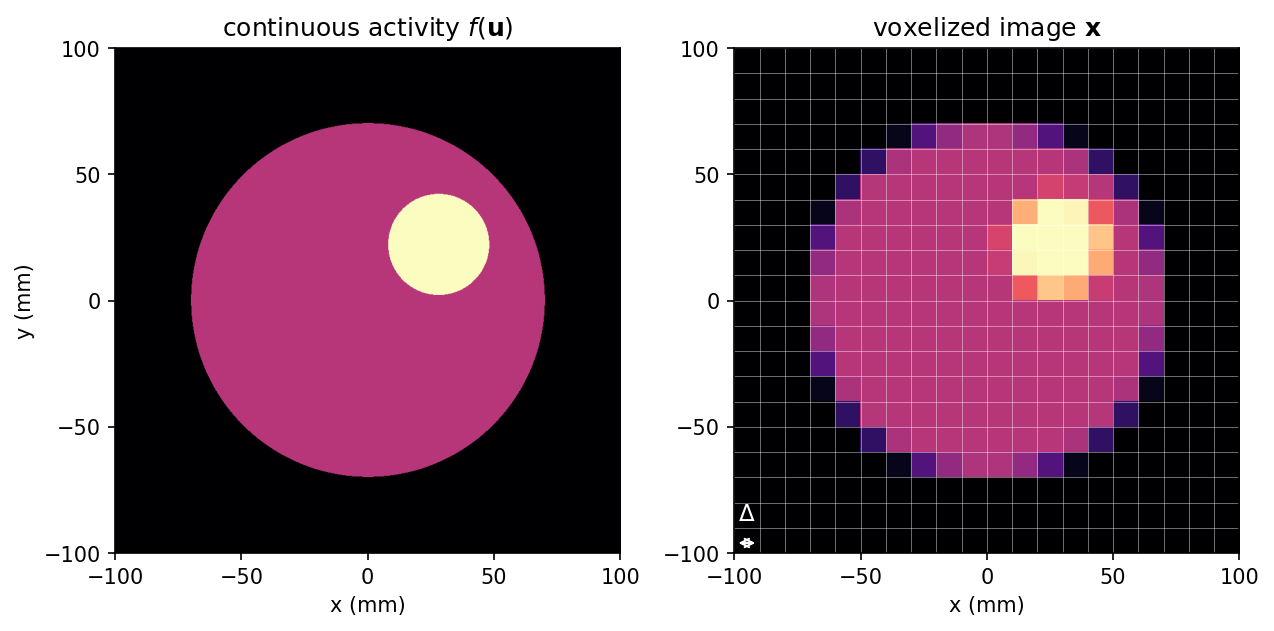
\includegraphics[width=0.92\textwidth]{figures/voxelization.png}
  \caption{Voxelization of the image. A continuous transverse activity
    distribution $f(\bm{u})$ (left) is represented on a voxel grid of spacing
    $\bm{\Delta}$ (right): each voxel carries a single value of $\xv$, and $f$ is
    recovered between voxel centres by trilinear interpolation. The grid is
    deliberately coarse here to make the voxels visible.}
  \label{fig:grid-voxelization}
\end{figure}

\subsection{Two roles of the voxel size}
\label{sec:grid:voxsize}

$\bm{\Delta}$ does double duty, and both matter. It \emph{places} the grid in
the world through \eqref{eq:grid-map}, converting voxel indices to millimetres
and back --- this is what lets a ray be intersected with the image box. And it
\emph{scales the line integral}: Joseph's method sums interpolated values over
voxel planes and multiplies by the path-length correction
$c=\Delta_{\mathrm{dir}}/\abs{\cos\theta_{\mathrm{dir}}}$
(Section~\ref{sec:projection:joseph}), with $\Delta_{\mathrm{dir}}$ the voxel
size along the ray's principal axis. A wrong voxel size therefore corrupts both
the geometry and the quantitative scale of the projection.

\subsection{Choosing the voxel size}
\label{sec:grid:resolution}

The voxel size controls how finely the image samples space; the spatial
resolution it can represent is set separately, by the detector and the data
(Section~\ref{sec:resolution}). The grid should be fine enough to sample that
resolution, which fixes a useful rule of thumb:
\begin{equation}
  \Delta \;\approx\; \tfrac13\ \text{to}\ \tfrac12\ \text{of the resolution }\FWHM .
  \label{eq:grid-sampling}
\end{equation}
At this spacing the grid captures the resolution the scanner delivers;
substantially coarser blurs it further, while much finer only inflates $N$ ---
and the reconstruction cost and the noise per voxel --- with no gain in detail.
The voxels need not be cubic: anisotropic $\bm{\Delta}$ is allowed, and is
natural when the axial sampling differs from the transverse. For a
$3.5\,\mathrm{mm}$-FWHM scanner such as CRYSP, \eqref{eq:grid-sampling} points to
roughly $1.2$--$1.8\,\mathrm{mm}$ voxels.

\subsection{Field of view}
\label{sec:grid:fov}

The grid should cover the region the scanner can image. Transversely the field
of view is bounded by the bore radius (which limits where LORs cross); axially it
is the ring span, or the axial field of view of a continuous scanner
(Section~\ref{sec:geometry}). Voxels well outside the measured LORs are crossed
by no ray: they accrue no sensitivity, and the reconstruction leaves them
untouched (Section~\ref{sec:mlem}). Sizing $\bm{n}\odot\bm{\Delta}$ to the field
of view, with the centred origin \eqref{eq:grid-center}, is the standard setup
the examples use.

% tbsrc/projection.tex — The Forward Model: Projection
% Status: written (first draft). Physics content migrated from the retired
% docs/tex/joseph3d_note.tex; port/implementation details live in the
% RecoCrysp Documenter pages, not here.
\section{The Forward Model: Projection}
\label{sec:projection}

The forward projector is the operator that turns an activity image into the
mean data the scanner would record. Section~\ref{sec:intro:problem} introduced
it abstractly as the system matrix $\Aop$ in $\pred = \Aop\,\xv$; this section
makes it concrete --- what $\Aop$ computes, how \code{RecoCrysp} evaluates it
with Joseph's method, and why its transpose $\Aadj$ must be the \emph{exact}
adjoint.

\subsection{The line integral and the system matrix}
\label{sec:projection:lineintegral}

Let $f(\bm{u})$ be the continuous activity field of
Section~\ref{sec:intro:problem}. In the idealized non-TOF model the expected
number of true coincidences on LOR $i$, with endpoints
$\bm{x}_s^{(i)}$ and $\bm{x}_e^{(i)}$
(Section~\ref{sec:geometry}), is the integral of $f$ along the line,
\begin{equation}
  p_i \;=\; \int_{\mathrm{LOR}_i} f(\bm{u})\,\mathrm{d}\ell .
  \label{eq:proj-lineintegral}
\end{equation}
The image is stored on a voxel grid (Section~\ref{sec:grid}) as the vector
$\xv\in\RR^N_{\ge0}$, and $f$ is reconstructed between grid points by
\emph{trilinear interpolation}; write $\tilde f$ for this interpolated field, so
that $\tilde f$ is linear in the voxel values $\xv$. Equation
\eqref{eq:proj-lineintegral} evaluated on $\tilde f$ is therefore linear in
$\xv$, and collecting all LORs gives the matrix form
\begin{equation}
  \pred \;=\; \Aop\,\xv ,
  \qquad
  \Aop \in \RR^{M\times N},
  \label{eq:proj-matrix}
\end{equation}
already met as \eqref{eq:intro-ideal}. Row $i$ of $\Aop$ holds the contribution
of each voxel to LOR $i$; it has only a handful of nonzeros (the voxels the ray
actually crosses), so $\Aop$ is extremely sparse. Crucially it is never formed:
\code{RecoCrysp} applies $\Aop$ and $\Aadj$ \emph{matrix-free}, recomputing the
weights on the fly for each LOR, which is what makes millions of LORs and
millions of voxels tractable.

\subsection{Joseph's method}
\label{sec:projection:joseph}

A direct evaluation of \eqref{eq:proj-lineintegral} would resample $\tilde f$ at
many points along each ray. Joseph's method~\cite{joseph1982} is a more
efficient and accurate quadrature that steps through the image one voxel plane
at a time. It first selects the \emph{principal axis} $d$ of the ray --- the
coordinate axis along which the ray travels fastest, i.e.\ the one with the
largest squared direction cosine,
\begin{equation}
  d \;=\; \argmax_{k\in\{1,2,3\}} \cos^2\theta_k ,
  \qquad
  \cos\theta_k \;=\; \frac{\Delta r_k}{\norm{\Delta\bm{r}}} ,
  \qquad
  \Delta\bm{r} \;=\; \bm{x}_e - \bm{x}_s .
  \label{eq:proj-principal}
\end{equation}
The integral is then approximated as a sum over the voxel planes perpendicular
to $d$,
\begin{equation}
  p_i \;\approx\; c \sum_{j=j_{\min}}^{j_{\max}}
      \mathcal{B}_d[\tilde f]\!\left(\bm{u}_j\right) ,
  \qquad
  c \;=\; \frac{\Delta_d}{\abs{\cos\theta_d}} ,
  \label{eq:proj-joseph}
\end{equation}
where $\mathcal{B}_d[\tilde f](\bm{u}_j)$ is the \emph{bilinear} interpolation
of the image within plane $j$, evaluated at the point $\bm{u}_j$ where the ray
pierces that plane, and $\Delta_d$ is the voxel size along $d$. Stepping along
the fastest axis guarantees that the ray crosses exactly one plane per voxel
step, so no plane is skipped or double-counted. Each plane contributes the
interpolated value sampled \emph{within} the plane (a $2\times2$ weighting),
while the geometric spacing between samples along the ray is folded into the
single \emph{path-length correction factor} $c$: the planes are a distance
$\Delta_d$ apart along $d$, but the ray segment between them is longer by
$1/\abs{\cos\theta_d}$, and $c$ converts the plane-by-plane sum back into a
length-weighted integral. Figure~\ref{fig:joseph} shows the construction.

\begin{figure}[t]
  \centering
  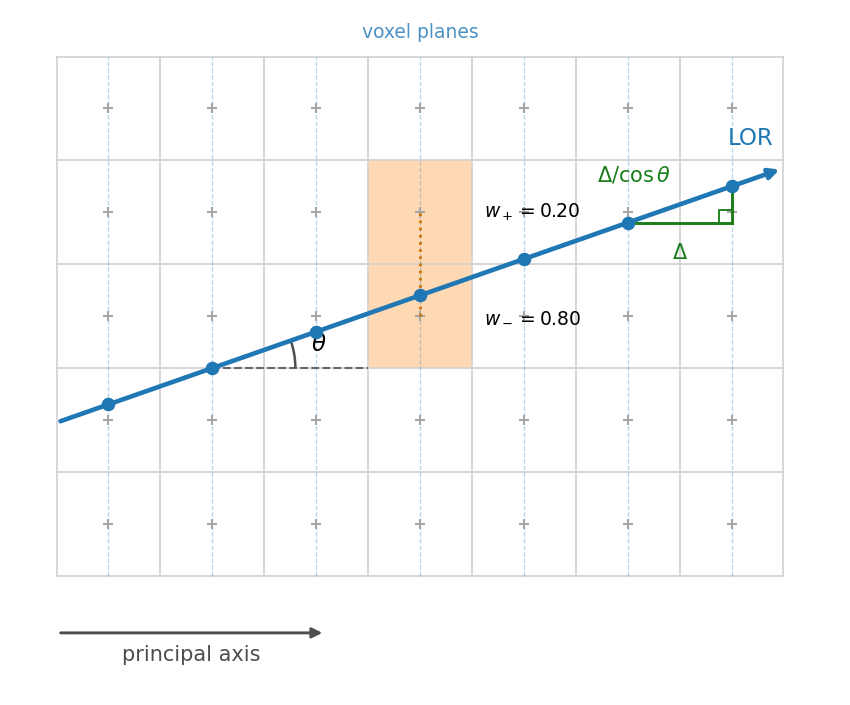
\includegraphics[width=0.82\textwidth]{figures/joseph_principle.png}
  \caption{Joseph's method (2D schematic). The ray's principal axis is
    horizontal; the method steps over the voxel planes perpendicular to it
    (dashed) and, at each crossing (dots), interpolates the image between the
    bracketing voxels with weights $w_\pm$ that sum to one (shaded column). The
    plane sum is then scaled by the correction factor $\Delta/\cos\theta$, the
    ratio of the ray segment between planes to their spacing $\Delta$. In 3D the
    in-plane interpolation is bilinear, over the four surrounding voxels.}
  \label{fig:joseph}
\end{figure}

Two properties make this cheap. The crossing points $\bm{u}_j$ advance by a
\emph{constant} increment from plane to plane, so the inner loop reduces to two
additions and one bilinear interpolation (four image samples) per plane. And
the traversal limits $j_{\min},j_{\max}$ follow from intersecting the ray with
the image bounding box, so only voxels actually on the ray are touched; rays
that miss the volume contribute zero.

\begin{remark}
The endpoints in \eqref{eq:proj-principal} are arbitrary world-space points, not
detector-element centres. The projector is therefore \emph{endpoint-driven}: it
integrates a thin line between whatever two points it is given and knows nothing
about crystal size or detector technology (Section~\ref{sec:geometry}). Finite
detector resolution is a separate operator $\Gop$, applied to the image before
projection (Section~\ref{sec:resolution}); it is deliberately not part of
$\Aop$.
\end{remark}

\subsection{Back-projection and the matched adjoint}
\label{sec:projection:adjoint}

Iterative reconstruction (Sections~\ref{sec:mlem}--\ref{sec:acceleration})
needs not only $\Aop$ but its transpose $\Aadj$, the \emph{back projector}.
Where the forward projector \emph{gathers} a value for each LOR from the voxels
it crosses, the back projector \emph{scatters} a per-LOR quantity $y_i$ back
into those same voxels:
\begin{equation}
  \bigl(\Aadj\,\yv\bigr)_v \;=\; \sum_i A_{iv}\,y_i .
  \label{eq:proj-back}
\end{equation}
\code{RecoCrysp} computes \eqref{eq:proj-back} by walking each ray exactly as in
the forward pass and adding $c\,y_i$ into the four bilinear voxels of every
plane, with the \emph{same} weights $A_{iv}$ used in the forward direction.
Because many LORs write to the same voxel, these updates are accumulated
atomically.

Using the identical weights in both directions is what makes the pair
\emph{matched}: $\Aadj$ is the true transpose of $\Aop$, so for any image $\xv$
and any data $\yv$,
\begin{equation}
  \inner{\Aop\,\xv}{\yv} \;=\; \inner{\xv}{\Aadj\,\yv} .
  \label{eq:proj-adjoint}
\end{equation}
This is not a cosmetic nicety. The convergence guarantees of MLEM and OSEM ---
that each iteration does not decrease the likelihood --- rest on $\Aadj$ being
the exact adjoint of the $\Aop$ used in the same update
(Section~\ref{sec:mlem}). An \emph{unmatched} projector/back-projector pair
(for instance a forward Joseph projector with a structurally different,
faster back projector) breaks \eqref{eq:proj-adjoint} and can stall or bias the
reconstruction. \code{RecoCrysp} therefore derives both directions from one
kernel and verifies \eqref{eq:proj-adjoint} numerically.

\subsection{Precision and validation}
\label{sec:projection:validation}

All projector arithmetic is single precision (\code{Float32}), matching the
reference implementation \code{parallelproj}~\cite{schramm2024} and the
requirements of the GPU backends (Section~\ref{sec:intro:scope}). Two checks pin
down correctness on every backend:
\begin{itemize}
  \item \textbf{Analytic line integrals.} An axis-aligned ray through a uniform
        image of $n$ unit voxels of size $\Delta$ must integrate to exactly
        $n\Delta$; \code{RecoCrysp} reproduces this to \code{Float32} machine
        precision.
  \item \textbf{Adjointness.} For random images and random LORs, the two sides
        of \eqref{eq:proj-adjoint} (accumulated in double precision for the
        comparison) agree to a relative deviation of order $10^{-10}$,
        confirming the back projector is the exact transpose.
\end{itemize}

In code, the two operators are a single call each: the LOR endpoints are passed
as $3\times M$ matrices and the grid as its origin and voxel size.
\begin{lstlisting}
proj  = joseph3d_fwd(xstart, xend, img, img_origin, voxsize)   # p = A x
bimg  = joseph3d_back(xstart, xend, proj, size(img), img_origin, voxsize) # A' y
\end{lstlisting}
The same source runs on multithreaded CPUs and on GPUs (including Apple Metal)
unchanged; the backend follows the array type of the arguments. These are the
building blocks every later section composes into a full reconstruction.

% tbsrc/resolution.tex — Detector Resolution and the Point-Spread Function
% Status: written (first draft). Blur sources; pixelated vs monolithic; the
% Gaussian PSF operator G; resolution injected at simulation time (not in the
% reconstruction), reconciling the forward model of Sec. projection/intro.
\section{Detector Resolution and the Point-Spread Function}
\label{sec:resolution}

The projector of Section~\ref{sec:projection} integrates infinitely thin lines:
it has no resolution of its own. Real PET data are blurred, and the previous
sections were careful to keep that blur out of the geometry. This section is
where it goes back in --- as a separate operator $\Gop$ --- and explains where,
in this tutorial, it enters the calculation.

\subsection{Sources of blur}
\label{sec:resolution:sources}

The spatial resolution of a PET scanner is limited by several physical effects,
none of which the reconstruction can undo by itself~\cite{moses2011}:
\begin{itemize}
  \item \emph{Positron range}: the positron travels a short distance before
        annihilating, so the annihilation is displaced from the emission ---
        sub-millimetre for $^{18}$F, larger for higher-energy emitters.
  \item \emph{Photon non-collinearity}: the two photons are not emitted exactly
        back to back (the pair carries residual momentum), spreading the angle
        by about $\pm0.25^\circ$; the resulting blur grows with the ring
        diameter, reaching a couple of millimetres in a human-scale scanner.
  \item \emph{Intrinsic positioning}: how well the detector localizes each
        photon interaction --- set by the crystal size for a pixelated detector,
        or by the readout and the position estimator for a monolithic one.
  \item \emph{Depth of interaction (DOI)}: photons enter the detector
        obliquely and interact at varying depth; without DOI information this
        smears the LOR, worsening off-centre (the parallax effect).
\end{itemize}
These contributions add approximately in quadrature to a total resolution,
quoted as a full width at half maximum ($\FWHM$). It is a property of the
scanner and the tracer, supplied to the model as data --- \code{RecoCrysp}
derives none of it.

\subsection{Pixelated versus monolithic detectors}
\label{sec:resolution:detectors}

The intrinsic term is where the two detector models of
Section~\ref{sec:geometry} differ sharply. A pixelated crystal of width $\ell$
localizes a photon only to within that crystal; a uniform uncertainty over a
width $\ell$ has standard deviation $\sigma=\ell/\sqrt{12}$, and the two
endpoints together give an intrinsic resolution of about $\ell/2$ FWHM at the
centre of the field of view. Resolution is thus tied to crystal size: finer
images demand smaller crystals, hence more readout channels.

A monolithic detector breaks this link. A large undivided block is read by a
photosensor array, and a neural network estimates the interaction position from
the light pattern; the accuracy is set by the light statistics and the network,
\emph{not} by the block size. CRYSP~\cite{crysp2026} reaches about
$3.5\,\mathrm{mm}$ FWHM with $50\,\mathrm{mm}$ blocks --- far finer than the
$\ell/2\approx25\,\mathrm{mm}$ a pixelated reading of the same block would give.
This decoupling is exactly why Section~\ref{sec:geometry:continuous} models the
detector as a continuous surface.

\subsection{The point-spread function as an operator}
\label{sec:resolution:psf}

Whatever its sources, the combined effect is that a point of activity is
recorded as a small blob: the system point-spread function (PSF). Over the
central field of view it is well approximated by an isotropic, spatially
invariant Gaussian of the total FWHM, which we write as a linear operator
$\Gop$ acting on the image --- convolution with that Gaussian,
\begin{equation}
  (\Gop\,\xv)(\bm u) = \int g(\bm u-\bm u')\,\xv(\bm u')\,\mathrm{d}\bm u' ,
  \qquad
  \sigma = \frac{\FWHM}{2\sqrt{2\ln 2}} \approx \frac{\FWHM}{2.355} ,
  \label{eq:res-gaussian}
\end{equation}
with $g$ the Gaussian of width $\sigma$. Like $\Aop$, $\Gop$ is applied without
forming a matrix; being a symmetric kernel it is self-adjoint, $\Gop=\Gop^{\mathsf T}$.
The resolution-aware forward operator is the composition $\Aop\,\Gop$, as
previewed in the full data model \eqref{eq:intro-full}. (The grid must sample
this Gaussian: this is the origin of the $\Delta\approx\tfrac13$--$\tfrac12\,\FWHM$
rule of Section~\ref{sec:grid:resolution}.) Treating the PSF as isotropic and
shift-invariant is an approximation --- real PSFs broaden towards the edge of
the field of view --- but an adequate one for the central-FOV examples here.

\subsection{Where the resolution enters}
\label{sec:resolution:where}

In this tutorial the resolution is injected \emph{at simulation time}, not in
the reconstruction. To generate realistic data for a known phantom
$\xv_{\mathrm{true}}$ we blur it and project the blurred image,
\begin{equation}
  \pred = \Aop\,(\Gop\,\xv_{\mathrm{true}}),
  \qquad
  \yv \sim \mathrm{Poisson}(\pred),
  \label{eq:res-sim}
\end{equation}
so the data $\yv$ carry the $3.5\,\mathrm{mm}$ blur. The reconstruction
(Section~\ref{sec:mlem}) then runs with the \emph{plain} projector $\Aop$.
Because the data are explained by $\Aop\,(\Gop\,\xv_{\mathrm{true}})$, the
iteration converges towards the blurred image $\Gop\,\xv_{\mathrm{true}}$: the
result is resolution-limited, resolving structures larger than the FWHM and not
those below it. This is the point of the resolution model --- one sees the limit
directly in the reconstructed image.

\begin{remark}
Equation~\eqref{eq:res-sim} is the \emph{image-space} way to inject resolution,
convenient because the phantom is known. A Monte-Carlo simulation does it the
\emph{detector} way instead --- jittering each LOR endpoint by the positioning
error, with no $\Gop$ operator at all. Both put the blur in the data, and the
reconstruction is identical. Building $\Gop$ \emph{into} the reconstruction
model (so that the iteration deconvolves towards $\xv_{\mathrm{true}}$) is
\emph{resolution recovery}: feasible with the same $\Gop$, but deliberately left
out of scope --- the examples reconstruct with $\Aop$ and report the
resolution-limited image.
\end{remark}

% tbsrc/datamodel.tex — Physical Effects: The Complete Data Model
% Status: STUB — to be written (see ../../PLAN.md for the planned content).
\section{Physical Effects: The Complete Data Model}
\label{sec:datamodel}
\textit{(Section to be written.)}

% tbsrc/statistics.tex — Statistical Model and the Likelihood
% Status: STUB — to be written (see ../../PLAN.md for the planned content).
\section{Statistical Model and the Likelihood}
\label{sec:statistics}
\textit{(Section to be written.)}

% tbsrc/mlem.tex — Iterative Reconstruction: MLEM
% Status: STUB — to be written (see ../../PLAN.md for the planned content).
\section{Iterative Reconstruction: MLEM}
\label{sec:mlem}
\textit{(Section to be written.)}

% tbsrc/acceleration.tex — Acceleration and Noise: OSEM and Semi-convergence
% Status: STUB — to be written (see ../../PLAN.md for the planned content).
\section{Acceleration and Noise: OSEM and Semi-convergence}
\label{sec:acceleration}
\textit{(Section to be written.)}

% tbsrc/regularization.tex — Regularized Reconstruction: MAP-EM
% Status: written (first draft). Follows the "Beyond early stopping" note in
% acceleration.tex. MAP objective f + beta R; De Pierro surrogate -> closed-form
% penalized_mlem for quadratic priors (intensity, smoothness); OSL -> osl_mlem for
% edge-preserving (Huber). Matches src/penalized.jl; De Pierro derivation in App.B.
\section{Regularized Reconstruction: MAP-EM}
\label{sec:regularization}

Early stopping (Section~\ref{sec:acceleration:reg}) controls noise by halting the
unregularized iteration before it fits the Poisson realization; it is blunt
because one global iteration budget governs every region irrespective of its
local statistics. The explicit alternative is \emph{maximum a posteriori} (MAP)
reconstruction: minimize the penalized objective
\begin{equation}
  \Phi(\xv) \;=\; f(\xv) \;+\; \beta\,R(\xv),
  \label{eq:reg-map}
\end{equation}
where $f$ is the negative Poisson log-likelihood of \eqref{eq:st-listmode}, $R$ is
a prior penalizing roughness, and $\beta\ge0$ sets its strength ($\beta=0$
recovers MLEM). The preconditioned-gradient view of Section~\ref{sec:mlem} makes
this a small change in principle --- the prior's gradient simply adds to
$\nabla f$ --- but the multiplicative update earns its non-negativity and
monotonicity from the EM structure, and naively bolting a gradient onto it forfeits
both. This section gives the two updates RecoCrysp implements in
\code{penalized.jl} that keep what the EM structure provides: a closed-form,
monotone update for \emph{quadratic} priors (De Pierro), and a One-Step-Late update
for \emph{edge-preserving} priors (Huber).

\subsection{Quadratic priors and the De Pierro update}
\label{sec:reg:depierro}

The obstacle is that $R$ couples neighbouring voxels, so its gradient mixes them
and the per-voxel decoupling that gave MLEM its closed form (Appendix~\ref{app:em})
is lost. De Pierro's surrogate~\cite{depierro1995} restores it: for a
\emph{quadratic} $R$, a convexity argument (Appendix~\ref{app:depierro}) replaces
the coupled penalty by a separable upper bound that is exact at the current
iterate, so the M-step again solves one independent problem per voxel --- now a
quadratic rather than a linear equation. Writing the ordinary EM numerator
\begin{equation}
  \\bm{t} \;=\; \xv_k \,\odot\, \Aadj\!\Bigl(\code{mult}\odot\frac{\code{counts}}{\pred_k}\Bigr)
  \label{eq:reg-numerator}
\end{equation}
(the quantity MLEM divides by $\sensv$), the penalized M-step is the positive root
of the per-voxel quadratic $G\,x^2 + B\,x - t = 0$,
\begin{equation}
  \xv_{k+1} \;=\; \frac{2\,\\bm{t}}{\sqrt{B^2 + 4\,G\,\\bm{t}}\;+\;B},
  \label{eq:reg-depierro}
\end{equation}
where the prior enters \emph{only} through the coefficients $(B,G)$, listed in
Table~\ref{tab:reg-priors}. The form makes the reduction to MLEM transparent: with
$\beta=0$ the prior contributes $G=0$ and $B=\sensv$, and \eqref{eq:reg-depierro}
collapses to $\xv_{k+1}=\\bm{t}/\sensv$, exactly \eqref{eq:ml-em}. The root is taken
in the rationalized form $2t/(\sqrt{B^2+4Gt}+B)$ rather than
$(-B+\sqrt{B^2+4Gt})/(2G)$ so that it stays well-defined as $G\to0$.

\begin{table}[t]
  \centering
  \begin{tabular}{@{}lll@{}}
    \toprule
    Prior $R(\xv)$ & $B$ & $G$ \\
    \midrule
    none (MLEM)
      & $\sensv$ & $0$ \\[2pt]
    intensity $\tfrac{\beta}{2}\norm{\xv-\bm z}^2$
      & $\sensv-\beta\,\bm z$ & $\beta$ \\[2pt]
    smoothness $\tfrac{\beta}{2}\sum_j\sum_{k\in\mathcal N_j}(x_j-x_k)^2$
      & $\sensv-\beta\,(\bm w\odot\xv_k+\bm m)$ & $2\beta\,\bm w$ \\
    \bottomrule
  \end{tabular}
  \caption{De Pierro coefficients $(B,G)$ for \eqref{eq:reg-depierro}, one entry
    per prior in \code{penalized.jl}. For the smoothness prior $\mathcal N_j$ is
    the 6-connected (face) neighbourhood, $\bm m_j=\sum_{k\in\mathcal N_j}x_k$ the
    neighbour sum, and $\bm w_j=\abs{\mathcal N_j}\in\{3,\dots,6\}$ the in-bounds
    neighbour count, both evaluated at the current iterate $\xv_k$. Every row
    reduces to $(\sensv,0)\Rightarrow$ MLEM at $\beta=0$.}
  \label{tab:reg-priors}
\end{table}

Two quadratic priors are provided. The \code{QuadraticIntensityPrior}$(\beta,\bm
z)$ pulls the image toward a reference $\bm z$; it is De Pierro's example prior and
serves mainly as a baseline, since penalizing intensity biases the activity. The
\code{QuadraticSmoothnessPrior}$(\beta)$ is the noise-controlling one: it penalizes
squared differences across the 6-connected neighbourhood, so its gradient is a
discrete Laplacian and the prior acts as a smoother. Because the De Pierro update
is the exact M-step of a surrogate that majorizes $\Phi$ and touches it at $\xv_k$,
it is \emph{monotone} --- $\Phi(\xv_{k+1})\le\Phi(\xv_k)$ at every iteration ---
inheriting the convergence guarantee MLEM has for the likelihood alone.

The neighbour sums $\bm m$ and counts $\bm w$ are the only new computation, and
they are a stencil over the image --- the same kind of structured, embarrassingly
parallel operation as the Joseph projector. They are written as a
KernelAbstractions kernel so the one source runs on CPU or GPU
(Section~\ref{sec:acceleration}), mirroring the projector idiom:
\begin{lstlisting}
@kernel function _neigh6_kernel!(nsum, wsum, @Const(x), n)
    I = @index(Global, Cartesian)
    i, j, k = I[1], I[2], I[3]
    s = 0.0f0; w = 0.0f0
    if i > 1;    s += x[i-1,j,k]; w += 1.0f0; end   # ... 5 more faces
    if i < n[1]; s += x[i+1,j,k]; w += 1.0f0; end
    nsum[I] = s; wsum[I] = w
end
\end{lstlisting}
The De Pierro iteration is then \eqref{eq:reg-numerator}--\eqref{eq:reg-depierro}
verbatim, with the prior reduced to its $(B,G)$ pair:
\begin{lstlisting}
B, G  = _prior_BG(prior, x, sens)               # Table 1; NoPrior -> (sens, 0)
denom = sqrt.(B.^2 .+ 4f0 .* G .* t) .+ B
x     = ifelse.(sens .> 0f0, 2f0 .* t ./ denom, x)   # leave FOV-exterior fixed
x     = max.(x, 0f0)                                  # guard Float32 cancellation
\end{lstlisting}
This is \code{penalized\_mlem}; called with \code{NoPrior()} it is bit-for-bit the
MLEM of Section~\ref{sec:mlem}.

\subsection{Edge-preserving priors: One-Step-Late}
\label{sec:reg:osl}

A quadratic smoothness prior penalizes \emph{every} difference equally, so it
blurs genuine edges along with noise. Edge-preserving priors penalize small
differences quadratically but large ones only linearly, leaving true boundaries
intact; the Huber penalty $\rho_\delta$ --- quadratic for $\abs t\le\delta$, linear
beyond --- is the canonical choice. Such priors are not quadratic, so the De Pierro
closed form does not apply. RecoCrysp uses instead the One-Step-Late (OSL) update
of Green~\cite{green1990}, which evaluates the penalty gradient at the
\emph{current} iterate and adds it to the sensitivity in the MLEM denominator:
\begin{equation}
  \xv_{k+1} \;=\; \frac{\\bm{t}}{\sensv + \nabla R(\xv_k)},
  \qquad
  \bigl(\nabla R\bigr)_j = \beta\!\!\sum_{k\in\mathcal N_j}\!\psi_\delta(x_j-x_k),
  \quad
  \psi_\delta(t)=\operatorname{clamp}(t,-\delta,\delta).
  \label{eq:reg-osl}
\end{equation}
The clamped influence $\psi_\delta$ is the Huber gradient: below $\delta$ it is the
identity, so the prior smooths like the quadratic one; above $\delta$ --- at an
edge --- it saturates, so the penalty stops pulling across the boundary and the
edge survives. The gradient is the same 6-neighbour stencil as before with
\code{clamp} in place of the bare difference, and $\beta=0$ again recovers MLEM.
OSL is the standard MLEM-structured edge-preserving scheme, but because the penalty
gradient is taken one step late it is \emph{not} provably monotone: it is stable at
the moderate $\beta$ used in practice and can diverge at very large $\beta$, so we
lean on $\beta=0\equiv$ MLEM as the anchor and verify behaviour empirically. For
quadratic priors \code{penalized\_mlem} (monotone) is preferred; \code{osl\_mlem}
is for the non-quadratic, edge-preserving case.

\subsection{Choosing the strength}
\label{sec:reg:beta}

The regularization weight $\beta$ has no universal value: it trades resolution
against noise, and because the prior is added to $f$ it must be commensurate with
the magnitude of $\sensv$, which depends on the geometry, the multiplicative
factors, and the event-to-sensitivity scale (Section~\ref{sec:datamodel}). On the
worked NEMA study (Part~II) $\sensv$ is of order $10^2$--$10^3$, so useful
smoothness/Huber strengths fall in $\beta\sim\mathcal O(10^2$--$10^3)$ and the Huber
threshold $\delta$ is set just above the noise scale of the differences;
both are tuned per study, like the iteration count. The practical finding there is
that for low-contrast features a quadratic smoothness prior, an edge-preserving
Huber prior, and a simple Gaussian post-filter on an early-stopped MLEM all sit on
nearly the same resolution--noise frontier --- regularization \emph{bounds} the
noise growth that early stopping merely outruns, and which of these realizations is
used matters little. Edge preservation pays off only where the features carry
strong edges for the Huber threshold to protect. The detailed comparison is the
subject of Part~II.

% tbsrc/pipeline.tex — The Reconstruction Pipeline
% Status: written (first draft). The skeleton common to every worked example:
% a calibration phase (events, mult, contamination, sensitivity) computed once,
% then a reconstruction phase that iterates mlem/osem and is monitored/stopped.
\section{The Reconstruction Pipeline}
\label{sec:pipeline}

The previous sections built every piece of a reconstruction; this one assembles
them into the workflow the worked examples all share. Underneath the different
phantoms and physics, each example is the same two-phase pipeline: a
\emph{calibration} phase that prepares the model inputs once, and a
\emph{reconstruction} phase that iterates. Naming this skeleton is what lets the
examples differ in their data while reusing identical reconstruction code.

\subsection{Calibrate once, iterate many times}
\label{sec:pipeline:twophase}

The objective \eqref{eq:st-listmode} and the MLEM update \eqref{eq:ml-em} read
from four inputs: the event geometry (LOR endpoints), the multiplicative factor
$\code{mult}=\nrm\odot\att$, the additive background
$\code{contamination}=\sct+\rnd$, and the sensitivity image
$\sensv=\Aadj(\code{mult})$. The decisive observation is that \emph{none of these
depends on the activity estimate} $\xv_k$: they are fixed by the scanner and the
object, not by the iterate. So they are computed once, before iterating, and
reused at every step --- and across solvers and datasets, exactly as the OSEM
example shares one $\sensv$ between MLEM and OSEM and between its sharp and
smeared acts. Only the predicted counts $\pred_k$ are recomputed each iteration,
through one forward projection of the current image.

\subsection{The calibration phase}
\label{sec:pipeline:calib}

Calibration turns the geometry and the physical maps into the four inputs. The
events are the listmode LOR endpoints --- read from the scanner for real data, or
sampled on the cylinder for a simulation (Section~\ref{sec:geometry}).
Attenuation comes from projecting the $\mu$-map, $\att=\exp(-\Aop\bm\mu)$
(Section~\ref{sec:datamodel}); normalization $\nrm$ and the background
$\sct+\rnd$ come from external calibration or models. The sensitivity image is
then the back-projection of $\code{mult}$ over the geometric LORs, computed once:
\begin{lstlisting}
xs, xe = sample_lors(scanner, nlors; rng = rng)     # or: read from acquisition
a      = exp.(-joseph3d_fwd(xs, xe, mumap, org, vs))     # attenuation a = exp(-A mu)
mult   = n .* a                                          # n = 1 for the examples
sens   = sensitivity_image(xs, xe, shape, org, vs; weights = mult)   # A^T(mult), once
\end{lstlisting}
In a simulation this phase also generates the data: project the (optionally
blurred) activity, scale to the desired count level, and draw Poisson counts,
\begin{lstlisting}
ybar   = mult .* joseph3d_fwd(xs, xe, gaussian_blur(x_true, fwhm, vs), org, vs) .+ s_plus_r
counts = [rand(rng, Poisson(c)) for c in ybar]
\end{lstlisting}
with $\Gop=\mathbf I$ (no blur) when resolution is switched off. For real data the
counts are simply the recorded events, and everything downstream is identical.

\subsection{The reconstruction phase}
\label{sec:pipeline:recon}

With the inputs prepared, reconstruction assembles the Poisson model and iterates.
The model carries the events, counts, $\code{mult}$, $\code{contamination}$ and
$\sensv$; MLEM (or OSEM, building subset models) runs from a positive image on the
sensitivity support:
\begin{lstlisting}
model = ListmodePoissonModel(xs, xe, sens; img_origin = org, voxsize = vs,
                             counts = counts, mult = mult, contamination = s_plus_r)
x0  = Float32.(sens .> 0)
rec = mlem(model, x0; niter = niter)                       # or osem(subset_models(...), x0)
\end{lstlisting}
This is the whole reconstruction. The physics lives entirely in the prepared
inputs; the solver is generic, which is why switching on attenuation, resolution,
or a background changes only the calibration phase, never these lines.

\subsection{Monitoring and stopping}
\label{sec:pipeline:monitor}

Two quantities track the run. The negative log-likelihood
\code{neg\_log\_likelihood} must decrease monotonically under MLEM
(Section~\ref{sec:mlem}); a non-decrease signals a bug or numerical trouble, so it
is the basic sanity check, available on real data since it needs no truth. When a
reference image \emph{is} known --- the truth or the recoverable $\Gop\xv$ in a
simulation --- the error against it is the quality metric, and it is what reveals
semi-convergence: it falls, reaches a minimum, and rises as noise is fitted
(Section~\ref{sec:acceleration}). The iteration count is therefore not run to
convergence but chosen by early stopping, a reconstruction parameter tuned per
study. The worked examples instrument exactly these quantities --- monotone
likelihood, error against the recoverable target, and the central-slice image ---
and report them alongside each reconstruction.

% tbsrc/summary.tex — Summary and the Example Ladder
% Status: written (first draft). Recap of the Part I arc around the data-model
% spine; the example-ladder table (physics rows) and the distinct solver axis;
% forward pointer to the remaining backgrounds.
\section{Summary and the Example Ladder}
\label{sec:summary}

Part~I built one equation and the algorithm that inverts it. The mean counts on
LOR $i$,
\begin{equation}
  \pred_i \;=\; n_i\,a_i\,\bigl(\Aop\,\Gop\,\xv\bigr)_i \;+\; s_i + r_i ,
  \label{eq:sum-spine}
\end{equation}
is the spine that every section hangs from: the geometry and grid fix what $\Aop$
means (Sections~\ref{sec:geometry}--\ref{sec:projection}), the resolution is
$\Gop$ (Section~\ref{sec:resolution}), the physical effects are $n,a,s,r$
(Section~\ref{sec:datamodel}), the Poisson statistics turn \eqref{eq:sum-spine}
into the likelihood (Section~\ref{sec:statistics}), and MLEM/OSEM minimize the
resulting objective (Sections~\ref{sec:mlem}--\ref{sec:acceleration}), assembled
into the two-phase pipeline of Section~\ref{sec:pipeline}. The library mirrors the
split: the multiplicative factors enter as $\code{mult}=\nrm\odot\att$, the
additive backgrounds as $\code{contamination}=\sct+\rnd$, the resolution is
injected at simulation time and left in the data, and the reconstruction needs
only these plus the sensitivity image $\sensv=\Aadj(\code{mult})$.

\subsection{The example ladder}
\label{sec:summary:ladder}

The worked examples (Part~II) switch the terms of \eqref{eq:sum-spine} on one at a
time, each isolating a single effect against everything before it already
working. Table~\ref{tab:ladder} is that ladder.

\begin{table}[h]
  \centering
  \begin{tabular}{@{}llllll@{}}
    \toprule
    Example & $\Gop$ & $\att$ & $\rnd$ & $\sct$ & what it isolates \\
    \midrule
    Attenuation & $\mathbf I$ & water $\mu$-map & $0$ & $0$ & cupping and its correction \\
    Resolution  & $5\,\mathrm{mm}$ & water & $0$ & $0$ & the blur $\Gop$, recovery of $\Gop\xv$ \\
    $+$ Randoms & $5\,\mathrm{mm}$ & water & flat & $0$ & a smooth additive background \\
    $+$ Scatter & $5\,\mathrm{mm}$ & water & flat & SSS/MC & object-dependent background \\
    \bottomrule
  \end{tabular}
  \caption{The physics example ladder. Each row adds one term of
    \eqref{eq:sum-spine} to the row above; normalization is $\nrm=\bm1$
    throughout (the continuous detector's geometric sensitivity is already in
    $\sensv$, Section~\ref{sec:datamodel}). The first two examples exist; randoms
    and scatter follow.}
  \label{tab:ladder}
\end{table}

The ladder is cumulative by design: because the reconstruction code is fixed
(Section~\ref{sec:pipeline}), turning on a term changes only how the data are
simulated, so each example's new effect is the \emph{only} thing that differs from
its predecessor and its consequence is unambiguous.

\subsection{A second axis: the solver}
\label{sec:summary:solver}

One worked example does not sit on this ladder. The acceleration example holds the
physics fixed --- it reuses the resolution phantom and attenuation --- and varies
the \emph{solver} instead, comparing MLEM with OSEM and exhibiting
semi-convergence. This is a genuinely different axis: the ladder switches on terms
of the forward model \eqref{eq:sum-spine}, while the solver study switches on
properties of the inversion (subset acceleration, the limit cycle, early
stopping). The two are orthogonal, which is exactly why the same generic
reconstruction runs every row of the ladder and every solver in the study.

\subsection{What follows}
\label{sec:summary:next}

The ladder's open rows are the additive backgrounds. Randoms add a smooth,
activity-independent term estimated from a delayed window; scatter adds a broad,
object-dependent term from an external single-scatter or Monte-Carlo model
(Section~\ref{sec:datamodel}). Both enter through \code{contamination} without
touching the reconstruction, completing the data model \eqref{eq:sum-spine} on
real-scale data. With geometry, resolution, attenuation, statistics, and the
solver in hand, those examples are the last step from the idealized forward model
to a quantitative reconstruction~\cite{crysp2026}.


\appendix
% tbsrc/appendices.tex — Appendices.  STATUS: STUB (after \appendix in driver).
\section{Expectation--Maximization derivation of MLEM}
\label{app:em}
\textit{(to be written: the complete EM derivation --- complete-data
likelihood, the $Q$-function, and the multiplicative update.)}

\section{Notation}
\label{app:notation}
\textit{(to be written: full glossary of symbols.)}

\section{RecoCrysp API quick reference}
\label{app:api}
\textit{(to be written: the functions and model fields used in the examples.)}


% tbsrc/references.tex — bibliography (self-contained, no bibtex step).
\begin{thebibliography}{9}

\bibitem{joseph1982}
P.~M. Joseph,
\emph{An improved algorithm for reprojecting rays through pixel images},
IEEE Trans.\ Med.\ Imaging \textbf{1}(3):192--196, 1982.

\bibitem{shepp1982}
L.~A. Shepp and Y.~Vardi,
\emph{Maximum likelihood reconstruction for emission tomography},
IEEE Trans.\ Med.\ Imaging \textbf{1}(2):113--122, 1982.

\bibitem{lange1984}
K.~Lange and R.~Carson,
\emph{EM reconstruction algorithms for emission and transmission tomography},
J.\ Comput.\ Assist.\ Tomogr.\ \textbf{8}(2):306--316, 1984.

\bibitem{hudson1994}
H.~M. Hudson and R.~S. Larkin,
\emph{Accelerated image reconstruction using ordered subsets of projection
data},
IEEE Trans.\ Med.\ Imaging \textbf{13}(4):601--609, 1994.

\bibitem{watson2000}
C.~C. Watson,
\emph{New, faster, image-based scatter correction for 3D PET},
IEEE Trans.\ Nucl.\ Sci.\ \textbf{47}(4):1587--1594, 2000.

\bibitem{moses2011}
W.~W. Moses,
\emph{Fundamental limits of spatial resolution in PET},
Nucl.\ Instrum.\ Methods Phys.\ Res.\ A \textbf{648}:S236--S240, 2011.

\bibitem{schramm2024}
G.~Schramm and K.~Thielemans,
\emph{PARALLELPROJ---an open-source framework for fast calculation of
projections in tomography},
Front.\ Nucl.\ Med.\ \textbf{3}:1324562, 2024.

\end{thebibliography}


\end{document}
